\clearpage{\pagestyle{empty}\cleardoublepage}
\chapter{Sviluppo dell'Infografica interattiva}

\section{Fase di Analisi}
\noindent In questa sezione verrà analizzata la creazione dell'infografica, partendo da alcuni mockup si cercheranno metodi per rendere il più efficiente e veloce possibile lo sviluppo.\newline
Verranno esposte delle considerazioni da tenere bene a mente durante quella che sarà la fase di sviluppo che verrà invece trattata a partire dalla sezione \ref{sec:svil}.
\subsection{Analisi dei Requisiti}
\noindent Scopo del progetto è la realizzazione di un'infografica interattiva in grado di mostrare dati e di fornire 
informazioni all'utente riguardo le importanti decisioni prese dall'Università di Bologna per favorire la digitalizzazione di alcuni processi per incrementare il risparmio della carta e quello conseguente di CO2 per aiutare l'ambiente.\newline
L'infografica verrà esposta principalmente su uno schermo pubblico, touchscreen multitouch 32" e Display FullHD (1920x1080px).\newline
Non sono stati forniti vincoli sugli strumenti da utilizzare.
Partendo dall’analisi dei mockup forniti, l’infografica interattiva è composta da una serie di pagine che si susseguono, in particolare:\newline
\begin{itemize}
    \item La pagina principale è sostanzialmente una vista sul Campus di Cesena dell’Università di Bologna. Per mostrare il campus all’interno del contesto, esso è posizionato su una collina verse con una serie di alberi decorativi. Il focus principale dell'infografica per ora è Cesena, ma Homepage alternative potranno essere sviluppate tranquillamente in futuro. Un footer si occuperà di dare informazioni generali sul progetto, una progress bar dovrà mostrare i nomi degli altri campus UniBo.
    \item Cliccando sul Campus accederemo alla seconda pagina, in cui appaiono le tre grandi categorie in cui è suddiviso il progetto: \textit{Comunicazione Digitale}, \textit{Dematerializzazione} e \textit{Innovazione del processo}.\newline
All'estrema sinistra ci dovrà essere un'altra progress bar, questa volta rappresentante gli anni solari da 2017 a 2020.
Questa progress bar comparirà anche in tutte le pagine seguenti. Quando si clicca su un anno le macro-categorie che in quel determinato anno non esistevano vengono nascoste.
Ogni macro-categoria è rappresentata da un albero o da un gruppo di alberi, da un'icona e dal proprio nome. Cliccando sugli alberelli otteniamo informazioni generali su quanti alberi sono stati salvati grazie ai progetti presenti in quella determinata categoria, oltre al quantitativo di CO$_2$ risparmiata. I dati sono relativi all'anno selezionato.\newline
A partire da questa pagina, anche tutte le successive conterranno una navigation bar da cui è possibile tornare alla pagina precedente. È anche presente l'icona del campus che è possibile cliccare per tornare più rapidamente alla homepage. L'icona dovrebbe cambiare in base al campus da cui è stato effettuato accesso.
\item Cliccando sulla categoria scelta si accede alla terza pagina, quella dei progetti. Ogni alberello in questa pagina rappresenta un determinato progetto della macro-categoria scelta. Ogni albero ha un nome, ossia quello del progetto che rappresenta. Il footer si occupa di dare informazioni sul progetto. Anche in questa pagina i progetti vengono nascosti se si sceglie un anno in cui ancora non esistevano.
\item Cliccando su un progetto (un alberello) si accede alla pagina finale. Il quantitativo di alberi salvati, di CO$_2$ risparmiata, di CO$_2$ assorbita e di fogli di carta risparmiati vengono riportati a schermo all'interno di alcuni grandi cerchi colorati. Ci sono esattamente quattro cerchi, uno per ogni informazione da mostrare:
\begin{itemize}
    \item[$\blacksquare$] numero di alberi salvati;
    \item[$\blacksquare$] numero di fogli di carta risparmiati;
    \item[$\blacksquare$] quantitativo di CO$_2$ risparmiata;
    \item[$\blacksquare$] quantitativo di CO$_2$ assorbita.
\end{itemize}
Il footer si occupa di dare informazioni sullo specifico progetto.\newline\newline
\end{itemize}

\noindent Non sono stati forniti mockup per quanto riguarda la versione mobile in quanto la versione mobile dell'infografica non era inizialmente requisito fondamentale.
L'approccio mobile first non è stato adottato per i seguenti motivi:
\begin{itemize}
    \item l'infografica verrà utilizzata principalmente e quasi esclusivamente tramite schermi pubblici sicuramente di tipo desktop;
    \item i mockup sono stati forniti solo in versione desktop;
    \item la versione mobile era inizialmente un requisito opzionale e non obbligatorio.
\end{itemize}
Grazie all'utilizzo di Bootstrap l'adattamento dell'infografica dalla versione desktop a quella mobile risulterà comunque non eccessivamente problematica.

\section{Sviluppo della Struttura dell'Infografica}
\label{sec:svil}
\noindent Lo sviluppo dell'infografica è stato suddiviso principalmente in due parti:
\begin{itemize}
    \item la creazione delle fondamenta dell'intero progetto e della struttura delle singole pagine statiche. In questa parte di sviluppo in altre parole è stato creato tutto ciò che è visibile, toccando più il lato front-end. Questa parte di sviluppo verrà trattata in questa sezione;
    \item la creazione della componente logica dell'infografica, ovvero lo sviluppo di tutto ciò che permette l'effettivo funzionamento di interazioni tra utente e sistema. Il problema verrà affrontato nella sezione \ref{sec:logic}.
\end{itemize}
\subsection{Struttura delle pagine}
\noindent La struttura delle pagine è sicuramente una delle parti che ha richiesto più tempo durante la fase di sviluppo.\newline
Il posizionamento delle immagini è stata probabilmente la parte più complicata da gestire.
L'applicazione è infatti molto dipendente dalle immagini e dal loro posizionamento, che deve essere rispettato indipendentemente dalle dimensioni dello schermo del visitatore.\newline
Per il posizionamento di alcune immagini è stato necessario utilizzare la proprietà \textit{position: absolute} invece delle classiche griglie offerte da Bootstrap. Sono infatti molte, da mockup, le immagini che hanno un posizionamento molto specifico.\newline
Ci sono inoltre casi in cui alcune grafiche sono sovrapposte. L'utilizzo della proprietà \textit{z-index: value} applicata alle immagini permette di specificare il livello di profondità in cui vengono inserite. \newline
Ogni pagina si deve adattare perfettamente alla dimensione dello schermo. Grazie all'inserimento della classe offerta da Bootstrap \textit{vh-100} è possibile fare in modo che l'applicazione non sorpassi mai l'altezza della finestra del browser in uso.\newline
Il componente utilizzato per creare il footer della homepage è riutilizzabile in tutte le altre pagine per mostrare le informazioni dei progetti e delle categorie. La struttura della parte inferiore di ogni pagina, lato grafico escluso, è infatti fortunatamente la stessa ovunque. Il componente React dedicato a questo compito si chiama \textit{DescriptionRow.js}.\newline
Anche la Navigation Bar nella parte superiore dello schermo è estremamente riutilizzabile in quasi ogni pagina. L'unica cosa che cambia è la stringa del pulsante che serve per tornare alla pagina precedente, facilmente personalizzabile tramite props.
Il nome assegnato al componente è \textit{TopBar.js}
\subsection{Utilizzo delle Librerie di terze parti}
\noindent La libreria Snap.svg è stata molto utile per la creazione dei cerchi informativi che dovranno contenere i dati relativi al servizio selezionato. I Componenti coinvolti sono \textit{Circle.js} e \textit{CircleContainer.js}.\newline
Il file CircleCointainer.js renderizza il contenitore dei quattro cerchi:
\begin{lstlisting}[language=Javascript]
    const idContainer = "svg-container";
    <svg viewBox={"0 300 1100 200"} height={"100%"} width={"100%"} id={idContainer}>
        [...]
    </svg>
\end{lstlisting}  
Inserendo una viewBox il contenitore e tutti i suoi figli saranno responsive.\newline
All'interno del contenitore vanno inseriti i componenti \textit{Circle}, segue l'inizializzazione di solo uno dei quattro:
\begin{lstlisting}[language=Javascript]
    let treeSavedLabel = "Alberi Salvati";
    let treeSaved = jsonObject["trees"];
    
    <Circle id={"c1"} x={210} y={300} containerId={idContainer} color={Colors.Green} radius={100}title={treeSaved} text={treeSavedLabel} textColor={Colors.White}/>
\end{lstlisting}
Le props più importanti sono \textit{x} e \textit{y} ovvero le coordinate del cerchio rispetto al contenitore.\newline
Il cerchio viene renderizzato utilizzando la sintassi di Snap.Svg quando il componente viene montato, ossia dentro la funzione \textit{componentDidMount()}.\newline\newline
Anime.js è stata utilizzata molto più di Snap.svg. Quasi ogni animazione dell'infografica è stata gestita utilizzando Anime.js.
La comparsa dei quattro cerchi della pagina finale per esempio avviene grazie al seguente codice:
\begin{lstlisting}[language=Javascript]
    <Anime initial={[{
                targets: 'svg g',
                duration: 5000,
                scale:[0,1],
                delay: stagger(DT_CIRCLE_APPEAR)}]}>
        [...]
    </Anime>
\end{lstlisting}

\noindent La struttura generale delle quattro pagine è stata creata. Accedendo con un browser da un ambiente desktop si ottengono le seguenti viste:
\begin{figure}[H]
    \centering
    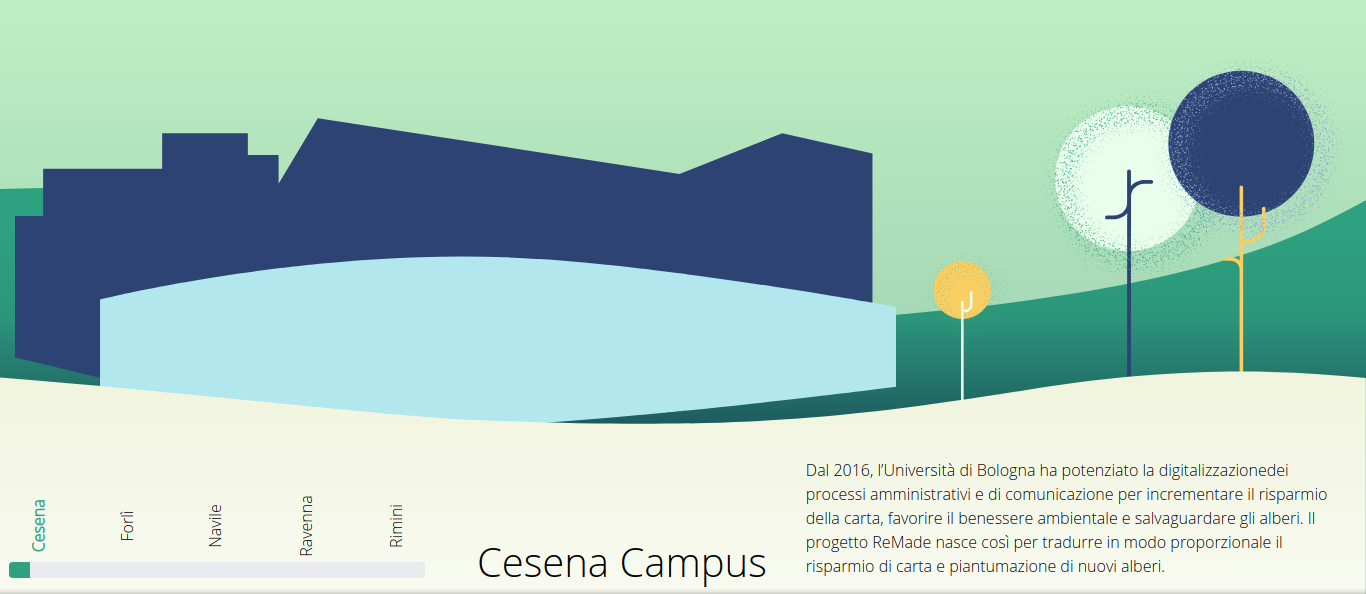
\includegraphics[width=0.9\linewidth]{img/first.png}
    \caption{Homepage (versione Desktop)}
    \label{fig:homeDesk}
\end{figure}

\begin{figure}[H]
    \centering
    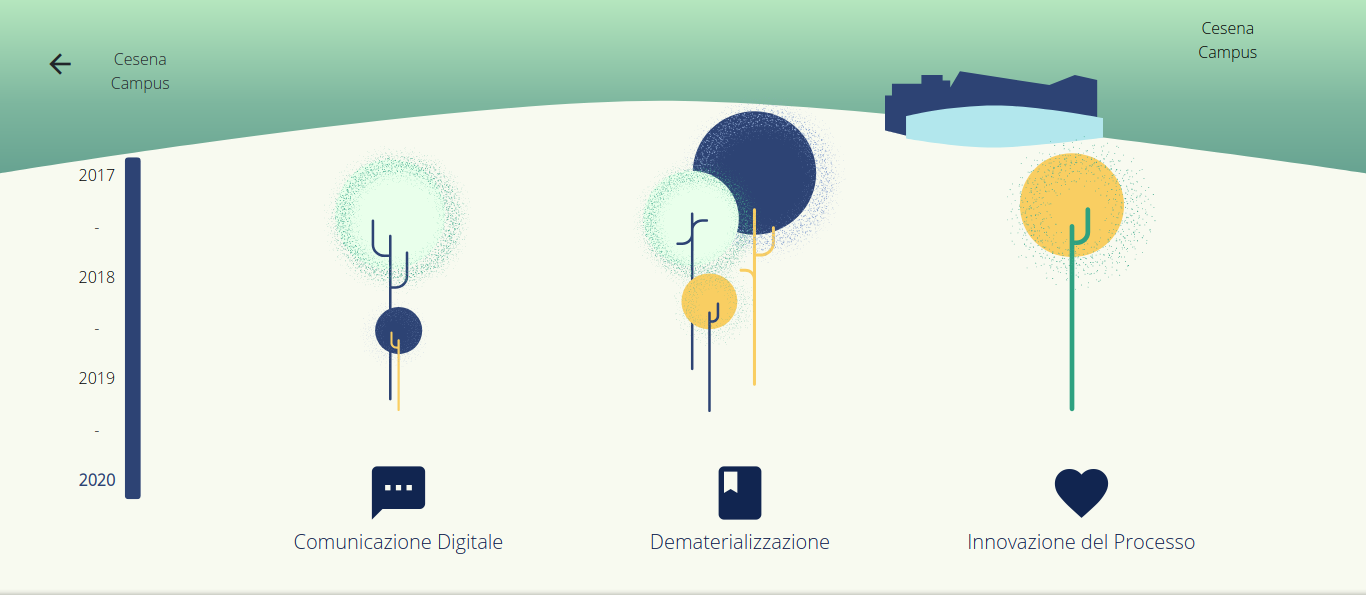
\includegraphics[width=0.9\linewidth]{img/second.png}
    \caption{Pagina delle Categorie (versione Desktop)}
    \label{fig:catDesktop}
\end{figure}

\begin{figure}[H]
    \centering
    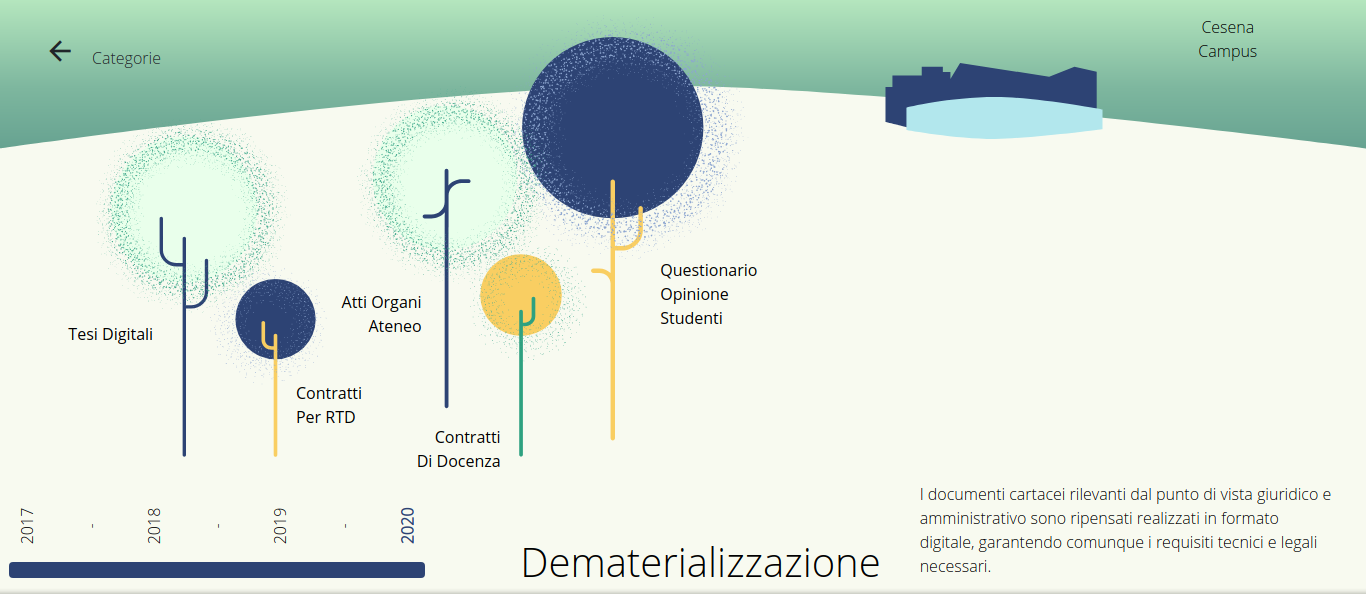
\includegraphics[width=0.9\linewidth]{img/third.png}
    \caption{Pagina dei progetti (versione Desktop)}
    \label{fig:projDesk}
\end{figure}

\begin{figure}[H]
    \centering
    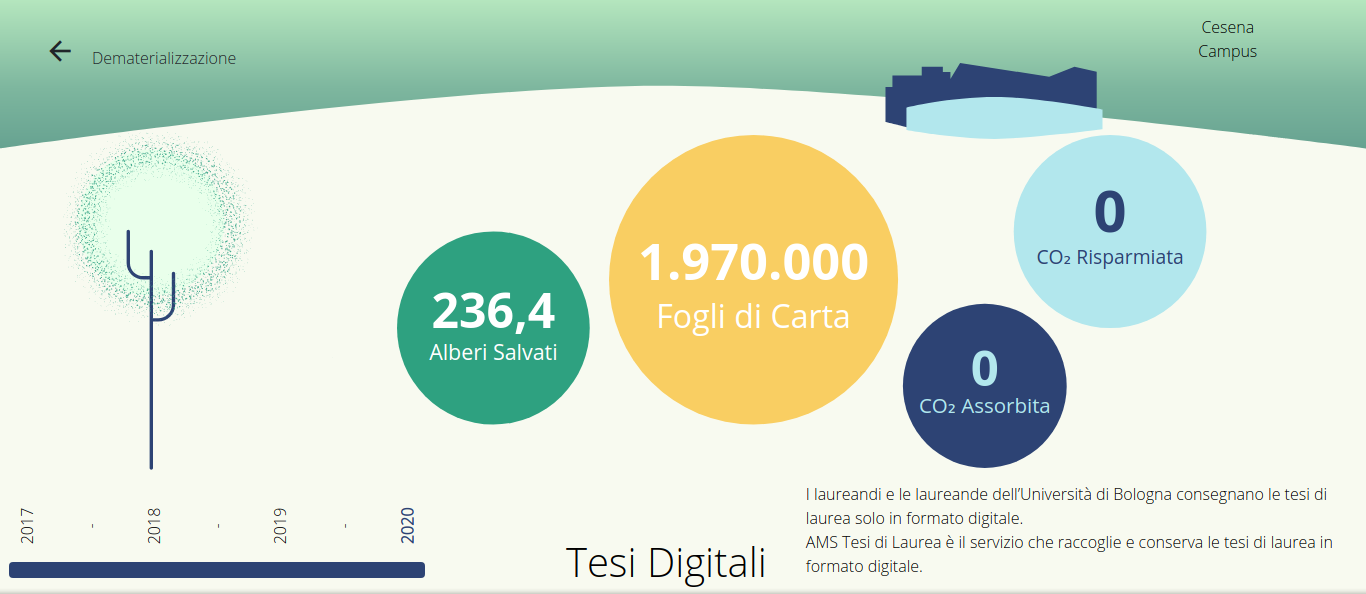
\includegraphics[width=0.9\linewidth]{img/fourth.png}
    \caption{Pagina del progetto selezionato (versione Desktop)}
    \label{fig:projSelDesk}
\end{figure}

\subsection{Struttura delle pagine (mobile)}
\noindent Come già anticipato la creazione della struttura delle pagine mobile è avvenuta solo una volta terminata la creazione della versione desktop.\newline
Tutte le pagine in versione desktop occupano tutta l'altezza della finestra grazie alla classe \textit{100-vh} fornita da Bootstrap. La versione Mobile è invece in formato scorrevole, in quanto sarebbe stato impossibile inserire tutti gli elementi della pagina nella singola schermata di un telefono.\newline
Dove possibile è stato sufficiente utilizzare le classi del Grid System di Bootstrap \cite{bootstrapGrid}. Il footer per esempio rimpicciolendo ogni pagina comincia ad impilare i propri componenti invece di affiancarli (Figure \ref{fig:footDesk} e \ref{fig:footMob}).
\begin{figure}[H]
    \centering
    
\includegraphics[width=\linewidth]{img/footer-desktop.png}
    \caption{Footer versione Desktop.}
    \label{fig:footDesk}
\end{figure}
\noindent Non tutto il progetto è gestito usando il Grid System. In casi estremi è stato necessario usare media query.
\begin{figure}[H]
    \centering
    
\includegraphics[width=0.5\linewidth]{img/footer-mobile.png}
    \caption{Footer versione Mobile.}
    \label{fig:footMob}
\end{figure}

\noindent Le viste mobile della Homepage e della pagina delle categorie sono rappresentate nelle figure \ref{fig:homepageMob} e \ref{fig:catMob}.


\begin{figure}[H]
\centering
\begin{minipage}{.5\textwidth}
  \centering
  
\includegraphics[width=.9\linewidth]{img/homepageMobile.png}
  \captionof{figure}{Homepage\\(versione Mobile)}
  \label{fig:homepageMob}
\end{minipage}%
\begin{minipage}{.5\textwidth}
  \centering
  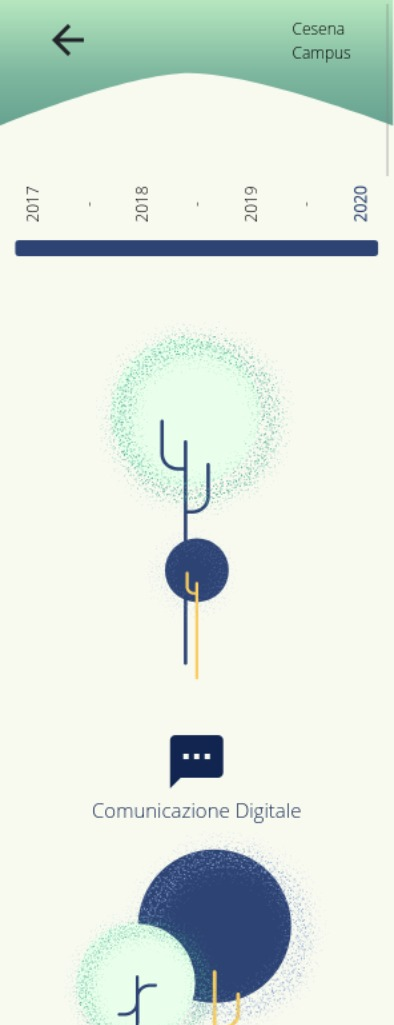
\includegraphics[width=.9\linewidth]{img/categoryMobile.png}
  \captionof{figure}{Pagine delle categorie (versione Mobile)}
  \label{fig:catMob}
\end{minipage}
\end{figure}

\section{Sviluppo della componente Logica}
\label{sec:logic}
\noindent In questa sezione verrà trattato lo sviluppo della parte back-end dell'infografica. Verranno inoltre illustrate le differenze tra state nativi e state globali. \newline
\subsection{Utilizzo degli state nell'Infografica}
\noindent In React gli state vengono utilizzati per gestire la logica interna dell'applicazione.\newline
In questa sottosezione verrà riportato un esempio di logica dell'applicazione: la comparsa dei dati al click degli alberelli nella pagina delle tre macro-categorie.\newline
Quando la pagina viene renderizzata la prima volta nessun alberello mostra i dati relativi alla propria categoria. Quando uno di essi viene cliccato mostra i proprio dati, che dovranno essere nascosti nel caso in cui un altro alberello sarà cliccato.\newline
Nel componente contenitore dei 3 alberelli è stato inizializzato il seguente costruttore:
\begin{lstlisting}
    constructor(props) {
        super(props);
        this.state = {
            treeSelected: -1
        };
    }
\end{lstlisting}
\noindent La funzione che si occupa di cambiare lo stato è implementata in modo estremamente semplice:
\begin{lstlisting}
    treeClick(treeClicked){
        this.setState({ treeSelected: treeClicked });
    }
\end{lstlisting}
Questa funzione viene chiamata quando viene cliccato uno degli alberelli. Il valore \textit{treeClicked} è ovviamente diverso per ognuno dei tre, i quali sono identificati da id progressivi (da 0 a 2).\newline
Quando l'albero viene renderizzato viene passata una props ``selected" booleana che controlla se il valore dello stato corrisponde a quello dell'albero.\newline
Se c'è corrispondenza vengono stampati anche i dati grazie alla renderizzazione condizionale.
\subsection{Utilizzo degli state Globali}
\noindent Gli state nativi di React sono spesso sufficienti per gestire la logica all'interno di qualsiasi pagina. A volte tuttavia uno stato potrebbe trovarsi ad un livello molto alto della gerarchia e numerosi componenti potrebbero aver bisogno di accedervi. Il passaggio degli state tramite props diventa dispendioso e molto complicato da gestire.\newline
La gestione del meteo e dell'ora della giornata (sottosezione \ref{sub:atm}) è possibile proprio grazie a due stati globali: \textit{``weather"} e \textit{``night"}.\newline
\textit{react-globally} \cite{reactGlobal} è una libreria disponibile su npm in grado di creare e gestire state globali. È sufficiente specificare gli stati globali all'interno del file \textit{index.js} e passarli tramite props ad un componente da inserire denominato \textit{Provider}.
\begin{lstlisting}[language=Javascript]
    const initialState = {
        weather: "Clear",
        night: false
    }
    
    ReactDOM.render(
        <Provider globalState={initialState}>
        [...] // App container
        document.getElementById('root')
    );
\end{lstlisting}
Quando da un qualsiasi componente si desidera cambiare il valore di uno stato globale è necessario usare la funzione \textit{setGlobalState()} invece della classica \textit{setState()}.
Inoltre quando si esporta il componente è necessario prima farne un wrapper utilizzando 
\begin{lstlisting}[language=Javascript, numbers=none]
export default withGlobalState(COMPONENT_NAME);
\end{lstlisting}
Lo state sarà poi accessibile dai componenti ed eventualmente assegnabile ad una variabile tramite la seguente sintassi:
\begin{lstlisting}[language=Javascript, numbers=none]
var global = this.props.globalState.stateName;
\end{lstlisting}

\label{sub:globalState}
\section{Sviluppo degli aspetti di Personalizzazione dell'Interfaccia}
\noindent In questa sezione verranno trattati elementi più di dettaglio non fondamentali per il funzionamento dell'interfaccia ma che rendono l'utente parte del campus di Cesena, a cui l'infografica fa riferimento, grazie ad informazioni strettamente legate ad esso come il meteo ed altre che vedremo in seguito.
\subsection{Gestione delle API}
\noindent L'infografica necessita di alcune informazioni particolari e non statiche per gestire alcuni aspetti grafici.
Nella sottosezione \ref{sub:atm} verranno illustrati due esempi che utilizzano chiamate API per modificare la HomePage per renderla più personalizzata.\newline
Il componente denominato \textit{Ticker.js} si occupa di effettuare chiamate API a tutti i servizi coinvolti.
Il meteo per esempio è offerto da OpenWeatherMap \cite{openWeather}. Creando un account sul portale si ottiene un token per poter effettuare un numero limitato di chiamate API (fino a un massimo di 60 all'ora)
La richiesta deve essere eseguita tramite GET all'indirizzo:\newline 
\url{http://api.openweathermap.org/data/2.5/weather?lat=LAT &lon=LON}
dove al posto di LAT e LON vanno inserite latitudine e longitudine della città interessata.\newline
La risposta da parte del server sarà ovviamente in formato JSON e sarà simile alla seguente (per semplicità sono stati omessi molti campi, è possibile trovare tutti i campi all'indirizzo \url{https://openweathermap.org/current}) \cite{openweatherGuide}:
\begin{lstlisting}[language=json, numbers=none]
    {
        "coord": { "lon": 139,"lat": 35},
        "weather": [{
            "id": 800,
            "main": "Clear",
            "description": "clear sky",
        }],
        [...]
    }
\end{lstlisting}
Il modo in cui verrà gestita questa risposta verrà illustrato in sottosezione \ref{sub:atm}.\newline
In React una richiesta API si può effettuare proprio come in Javascript nel seguente modo:
\begin{lstlisting}[language=Javascript]
    fetch(API_LINK)
        .then(response => response.json())
        .then(json => {
            // json is the json object in response
        }).catch((error) => {
        console.log("ERROR: (" + error + ")");
    });
\end{lstlisting}
Per ottenere gli orari di alba e tramonto la richiesta viene invece effettuata tramite GET al link \url{https://api.sunrise-sunset.org/json?lat=36.7201600&lng=-4.4203400}. A differenza di OpenWeatherMap, Sunrise-Sunset non necessita di un token e non ci sono limiti al numero di richieste effettuabili.
La risposta è nel formato seguente:
\begin{lstlisting}[language=json, numbers=none]
    {
      "results":
      {
        "sunrise":"7:27:02 AM",
        "sunset":"5:05:55 PM",
        [...]
      },
       "status":"OK"
    }
\end{lstlisting}
Tutti gli orari sono in formato UTC \cite{sunriseSunset}.\newline
All'interno di \textit{Ticker.js} per ogni servizio viene inizializzato un timer che richiama le funzioni che effettuano le chiamate API quando il componente viene montato.
\begin{lstlisting}
    componentDidMount() {
        this.timerID = setInterval( () => 
            this.tick(), //API function
            60000 //period
            );
    }
\end{lstlisting}
Ticker è un componente presente su ogni pagina. Tutte le richieste API possono essere eseguite indipendentemente da dove si trova il visitatore. Le informazioni come il meteo attuale o se è giorno o notte sono gestite attraverso Stati Globali (Sottosezione \ref{sub:globalState})
\subsection{Homepage personalizzata in funzione di ora e condizioni atmosferiche}
\label{sub:atm}
\noindent Una volta impostato lo stato globale della notte a true o false in funzione degli orari di alba e tramonto offerti dall'API è possibile personalizzare l'interfaccia.\newline
Utilizzando la renderizzazione condizionale sullo stato ``night" è possibile impostare un colore diverso per il cielo e far comparire nuovi elementi come il sole e la luna sulla schermata.
\begin{figure}[H]
    \centering
    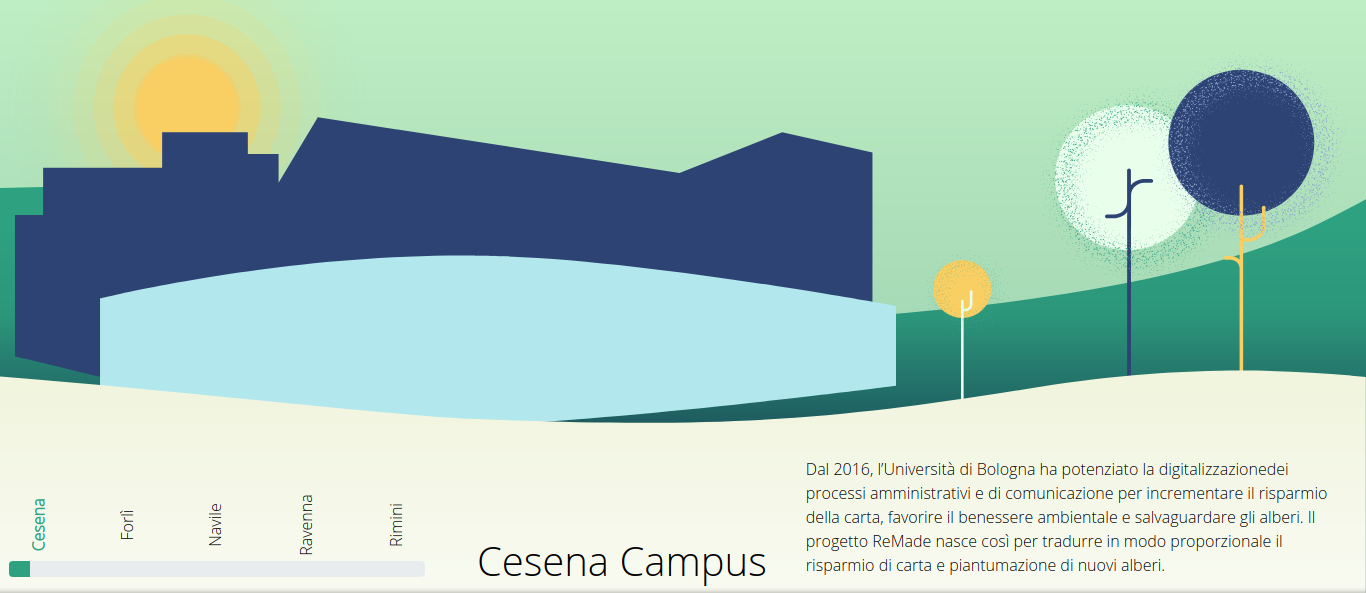
\includegraphics[width=\linewidth]{img/day.png}
        \caption{Homepage (Giorno)}
    \label{fig:day}
\end{figure}

\begin{figure}[H]
    \centering
    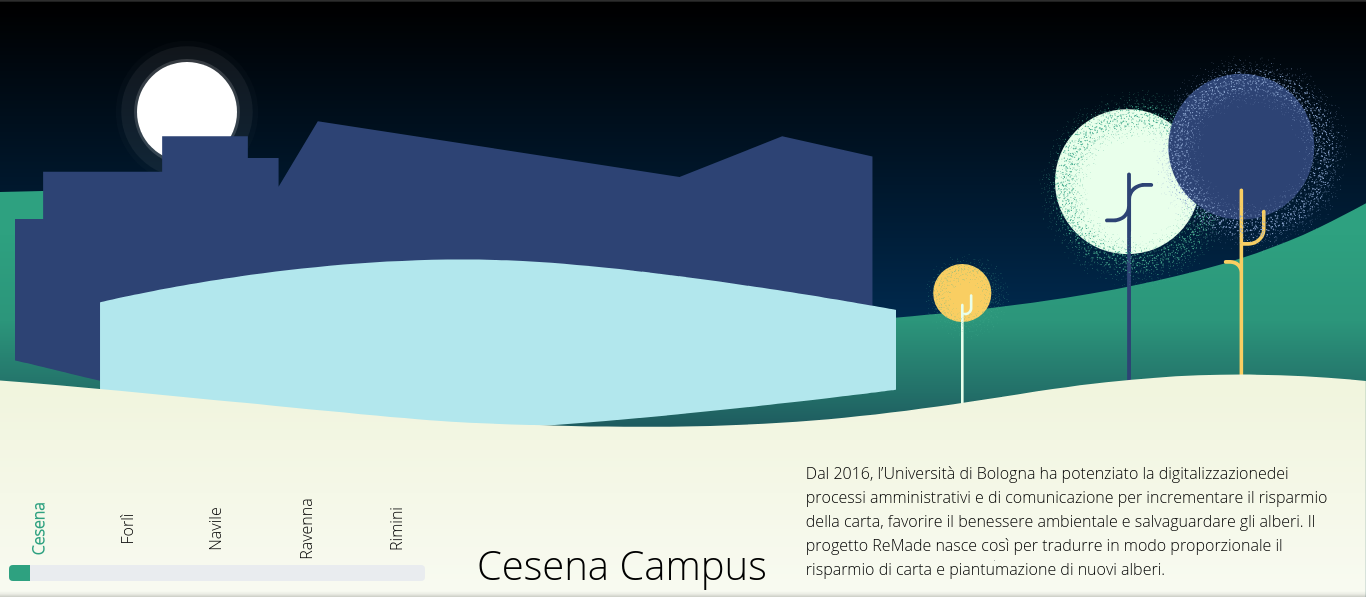
\includegraphics[width=\linewidth]{img/night.png}
        \caption{Homepage (Notte)}
    \label{fig:night}
\end{figure}

\noindent Nelle figure \ref{fig:day} e \ref{fig:night} vengono riportate le due schermate.
OpenWeatherMap mette a disposizione la lista completa di tutti i possibili tipi di meteo nella documentazione \cite{openweatherWeather}.
Il meteo sull'applicazione è stato ulteriormente semplificato e tutte le possibili condizioni atmosferiche si trovano dentro il file \textit{Weather.ts} sotto forma di Enumerated Type:
\begin{itemize}
    \item \textit{``Clear"} quando il tempo è sereno;
    \item \textit{``Clouds"} quando il tempo è nuvoloso;
    \item \textit{``Snow"} quando nevica o grandina;
    \item \textit{``Rain"} quando piove o c'è un temporale;
    \item \textit{``Fog"} quando c'è la nebbia o molto smog.
\end{itemize}
Se OpenWeatherMap fornisce indicazioni sul meteo lo state globale denominato weather viene impostato a uno dei valori dell'enum e la HomePage aggiornata di conseguenza.\newline
Se non si riesce ad contattare il servizio OpenWeatherMap il meteo viene impostato automaticamente a ``Clear".\newline
L'orario del giorno funziona in modo molto simile al meteo. Una volta ottenuti gli orari di alba e tramonto dall'apposita API un timer controlla ogni minuto se l'orario ricade nell'intervallo del giorno o in quello della notte. Lo state globale ``night" viene aggiornato quando si raggiunge uno dei due orari prestabiliti e l'interfaccia viene aggiornata di conseguenza.\newline\newline
La renderizzazione degli effetti meteo è gestita dal componente \textit{WeatherContainer.js}. Lo state globale weather viene passato dal componente al livello superiore a \textit{WeatherContainer.js} come props, il quale applica gli elementi del meteo alla Homepage grazie alla renderizzazione condizionale \cite{reactCond}.

\begin{figure}[H]
    \centering
    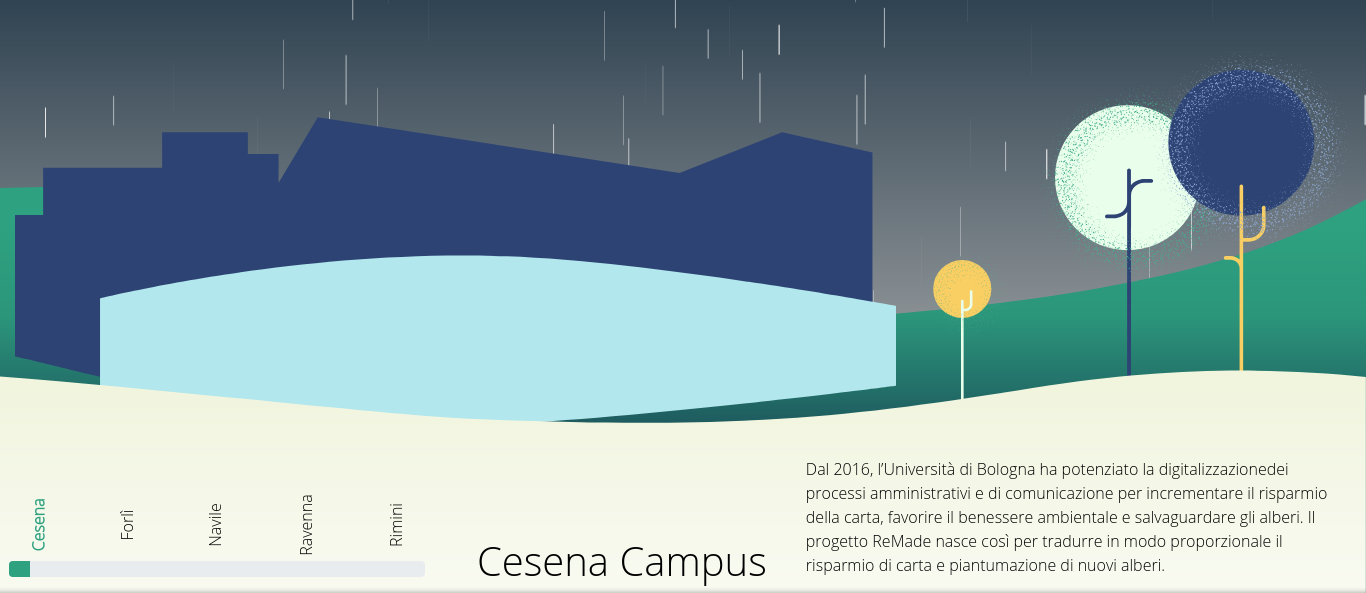
\includegraphics[width=\linewidth]{img/rain.png}
        \caption{Homepage (Pioggia)}
    \label{fig:dayrain}
\end{figure}

\begin{figure}[H]
    \centering
    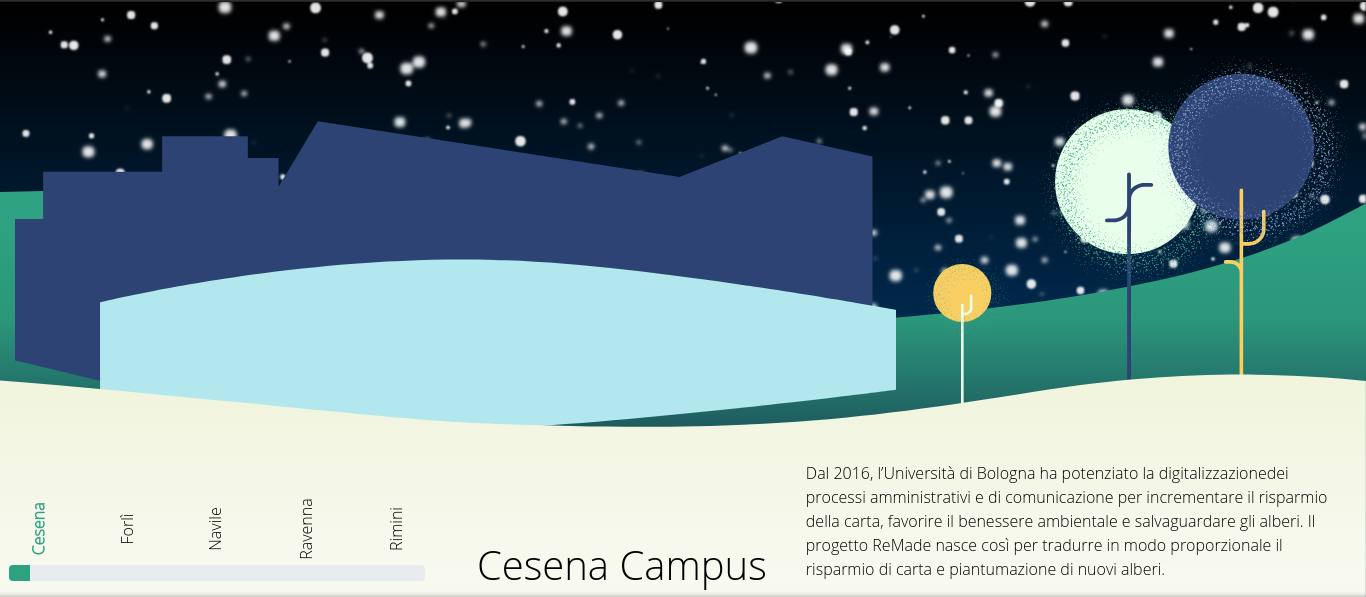
\includegraphics[width=\linewidth]{img/snow.png}
        \caption{Homepage (Neve e Notte)}
    \label{fig:nightsnow}
\end{figure}

\subsection{Integrazione di dati provenienti da Sensori}
\noindent Nell’infografica si vogliono anche mostrare dati provenienti da sensori Canarin II per informare l’utente su temperatura, pressione, umidità e qualità dell’aria all’esterno del campus di Cesena. Per ottenere questi dati, è stato necessario collegarsi ad un database esterno dove le informazioni sono salvate con i seguenti campi:
\begin{itemize}
\item \textbf{node\_id}: id del canarin da cui provengono i dati;
\item \textbf{value\_num}: il valore restituito dal sensore;
\item \textbf{type\_id}: l’id che indica il tipo di sensore; 
\item \textbf{timestamp}: data di rilevazione del dato.
\end{itemize}
Anche gli oggetti json restituiti avranno un formato simile. Invece di mantenere il dato \textit{type\_id} così com'è, nell'oggetto json ci sarà il campo \textit{type} che assumerà i seguenti valori in base al valore di \textit{type\_id}:

\begin{itemize}
    \item \textbf{temperature}: type\_id 37;
    \item \textbf{humidity}: type\_id 38;
    \item \textbf{pressure}: type\_id 6; 
    \item \textbf{pm 1.0}: type\_id 9;
    \item \textbf{pm 2.5}: type\_id 7;
    \item \textbf{pm 10}: type\_id 8.
\end{itemize}
\noindent Come per le condizioni atmosferiche esiste una enum anche per i tipi di dati dei sensori. In questo modo saranno più facili gestire informazioni come il nome del sensore da stampare a schermo e l'unità di misura del dato.\newline
I dati dei sensori vengono presentati sulla Homepage all'interno di una Bootstrap Card.
Inizialmente la Card viene posizionata nella parte in alto a destra dello schermo.
La Card è un oggetto draggable, è possibile cioè spostarla liberamente sullo schermo.\newline
Vengono mostrati solo i dati più recenti per ciascun tipo di sensore. I dati vengono recuperati tramite la relativa API ed eventualmente filtrati tramite Javascript.\newline
La Homepage finale, integrando anche i dati ottenuti dai sensori avrà il seguente aspetto:
\begin{figure}[H]
    \centering
    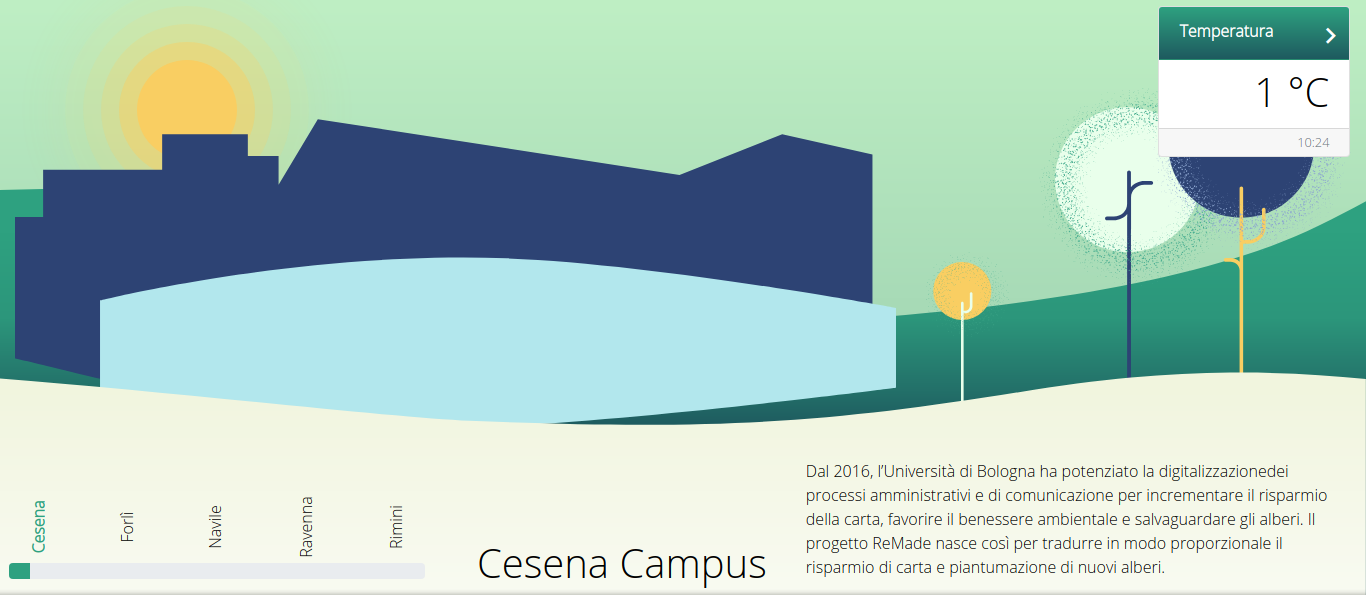
\includegraphics[width=\linewidth]{img/final.png}
        \caption{Vista sulla Homepage con integrazione dei dati dai sensori Canarin II.}
    \label{fig:final}
\end{figure}


